\RequirePackage{fixltx2e}
\documentclass[a4paper, titlepage, 12pt, twoside, open=right]{scrartcl}
\usepackage[utf8]{inputenc}  
\usepackage[T1]{fontenc}
\usepackage{mathtools}
\usepackage{longtable}
\usepackage{lmodern}           
\usepackage{polyglossia}
\usepackage{morewrites} %wtf
\usepackage{forest} % this is for the stemma diagram
\usepackage[onehalfspacing]{setspace}
\usepackage[toc,page]{appendix}
\usepackage{multirow,bigdelim}
\usepackage{parnotes}
\usepackage{xfrac}
\usepackage{graphicx}% stellt \scalebox bereit
\usepackage{array,booktabs}% für Tabellen
\usepackage{natbib}
\onehalfspacing
\setdefaultlanguage{english}
\usepackage{xeCJK}
 \setCJKmainfont[BoldFont=SimHei]{SimSun}
%\setCJKmainfont{Noto Sans CJK TC Regular}
\usepackage{marginnote}
\usepackage{geometry}           
\usepackage[multiple,perpage]{footmisc}
\usepackage{endnotes}
\def\enoteheading{\section{\notesname}%
\mbox{}\par\vskip-\baselineskip}
\geometry{left=2cm,right=3cm,top=2.5cm,bottom=2.5cm}
\usepackage{changepage}
\usepackage[hidelinks]{hyperref}
\usepackage{xcolor}

%avoid indent in quotes:
\makeatletter
\renewenvironment{quotation}
  {\list{}{\listparindent=1.5em
           \itemindent=0pt
           \parsep\z@ \@plus\p@}%
           \item\relax}
  {\endlist}
\makeatother


\begin{document}

\clearpage
\thispagestyle{empty}
\titlehead{}
\title{Through the Yellow Gate}
\subtitle{Ordination of Gender-Nonconforming People in Buddhism}
% \author{Ven. Vimala Bhikkhunī}
\author{DRAFT COPY}
\date{\today}
\maketitle

\tableofcontents
\newpage
\section{Introduction}
The legality of Bhikkhunī ordination in the Theravada and Tibetan lineages of Buddhism has been a hotly debated issue for many years. Thanks to the efforts and research of many monastics and academics, the first full Theravada ordination was held in Perth in October 2010 (\cite{sujato2009}, \cite{analayo2013}). Although still not widely recognized in several traditional Theravada countries, recognition is growing and the number of Bhikkhunīs is slowly increasing. 

There are however two groups of people that have been marginalized and excluded from ordination, groups which we will refer to here with the Pāli terms used in the Theravada Vinaya: {\em paṇḍaka} and {\em ubhatob­yañ­janaka}. There have been various translations and interpretations of these terms with the consequence that intersex people and transgenders have been barred from ordination. But there is also much ambiquity.

When studying the Buddhist scriptures, especially where there are groups of people who seem to be marginalized, it is important to understand where and under which circumstances these concepts and interpretations have originated. The Early Buddhist Texts mainly focus on the teachings themselves, and much less on the socio-cultural environment in which these originated. In fact, they seem to deal with sex and gender as a given, that need no further discussion. So we have to look elsewhere for more information on this topic, like the pre-Buddhist Vedic culture\footnote{Note that in this work I have deviated from some of the earlier points I made in \cite{vimala} with regards to the Vedic concept of the third sex. I have now rejected certain sources on the basis that I found them unreliable upon closer inspection and I hope to have rectified this with more thourough research.} and the Brahmanic and Jain cultures at the time of the Buddha and thereafter. 

The Jains were contemporaries to the Buddha and also shared the acceptance of a third sex, which led them to speculate what the nature of this third sex might be as compared to male and female. Just like in Buddhism, the Jain order had a strong interest in controlling the sexuality of it's monastics. Jain monastics live celibate and at the time of it's emergence, the monks were mostly naked ascetics. The prestige and power of the order depended to a large extend on public opinion and therefore on the purity of their behavior, as well as their external appearance. The "third sex" was therefore subject of a very lengthy debate within the order within a larger discussion on the nature of sexuality. The Jains left us a vast literature in Sanskrit and Prakrit in which these discussions and concepts are discussed in detail.
\newpage
\section{Appendix 1: Glossary of Definitions}
\label{appendix1}

\subsection{Definitions of Pāli words}
In this section I refer to the various dictionary definitions of the words relevant to the subject matter and provide links to these dictionaries.

\subsubsection{Napuṃsaka}
Pāli word: {\em napuṃsaka} \\
Pāli dictionary: \href{https://suttacentral.net/define/napu%E1%B9%83saka}{see SuttaCentral} \\
Sanskrit word: {\em napuṃsaka} \\
Sanskrit dictionary: \href{https://www.wisdomlib.org/definition/napumsaka}{see WisdomLib} \\

\subsubsection{Paṇḍaka}
Pāli word: {\em paṇḍaka} \\
Pāli dictionary: \href{https://suttacentral.net/define/pa%E1%B9%87%E1%B8%8Daka}{see SuttaCentral} \\
Sanskrit word: {\em paṇḍaka} \\
Tibetan word: {\em ma ning} or {\em ’dod ’gro} \\
Chinese word: {\em 種不能男} or {\em 黃門} (first one lit means 'neither male nor female'.\\
ITLR dictionary: \href{http://www.itlr.net/hwid:281142}{see itlr.net} \\

\subsubsection{Ubhatob­yañ­janaka}
Pāli word: {\em ubhatob­yañ­janaka} or {\em ubhatovyañ­janaka} \\
Pāli dictionary: \href{https://suttacentral.net/define/ubhatovya%C3%B1janaka}{see SuttaCentral} \\
Sanskrit word: {\em ubhayavyañjana} \\
Tibetan word: {\em mtshan gnyis pa} \\
ITLR dictionary: \href{http://www.itlr.net/hwid:62844}{see itlr.net} \\

\subsubsection{Other references}
There are various other words mentioned in the ordination procedures for Bhikkhunī as described in Bhikkhunikkhandhaka that might be interesting in this context. These do not excluse from ordination and have been translated by Ajahn Brahmali as follows: \\

\begin{tabular}{ l l }
 {\em animittā } & woman who lacks genitals \\
 {\em nimittamattā } & woman with incomplete genitals \\ 
 {\em vepurisikā } & woman who is manlike \\
\end{tabular} \\

The word {\em animittā} literally means 'signless' and appears a number of times in the canon (excluding commentaries) but mostly in a different meaning, namely as in {\em Animitto (ceto)samādhi}, which is translated by Bhikkhu Sujato as 'signless immersion', a term used in the context of meditation. In the context of not having genitals, it only appears in the canon in the Bhikkhunikkhandhaka and as a form of abuse for women in the Bhikkhu Saṃ­ghā­di­sesa­ 3, never on it's own but always in the same sequence of words of which the above are a few. This points towards a later development.


\subsection{Modern Definitions}
In this section I list a few terms relevant to the subject matter because there are many misunderstandings with regards to these terms and their meanings. For other terms, I refer to \href{https://www.hrc.org/resources/glossary-of-terms}{the website of the Human Rights Campaign}

\subsubsection{Intersex}
\label{intersex}
The definition of the term 'intersex' according to the \href{https://unfe.org/system/unfe-65-Intersex_Factsheet_ENGLISH.pdf}{UN Office of the High Commissioner for Human Rights} is as follows:

\begin{quote}
Intersex people are born with sex characteristics (including genitals, gonads and chromosome patterns) that do not fit typical binary notions of male or female bodies.

Intersex is an umbrella term used to describe a wide range of natural bodily variations. In some cases, intersex traits are visible at birth while in others, they are not apparent until puberty. Some chromosomal intersex variations may not be physically apparent at all.
\end{quote}

Intersex can be divided into 4 categories according to the \href{https://medlineplus.gov/ency/article/001669.htm}{US National Library of Medicine}:

\begin{tabular}{ l l }
46, XX intersex & female internal organs and chromosomes \\
& external genitals appear male \\
46, XY intersex & male internal organs and chromosomes \\
& external genitals appear female or ambiguous \\
True gonadal intersex & both ovarian and testicular tissue \\
& external genitals ambiguous or \\
& appear female or male \\
Complex or undetermined intersex & chromosomes discrepancies only \\
\end{tabular}


\subsubsection{Hermaphrodite}
\label{hermaphrodite}
A hermaphrodite is an organism that has both male and female reproductive organs. Until the mid-20th century, 'hermaphrodite' was used synonymously with 'intersex'. The distinctions 'male pseudohermaphrodite', 'female pseudohermaphrodite' and especially 'true hermaphrodite' are terms no longer used, which reflected histology (microscopic appearance) of the gonads. Medical terminology has shifted not only due to concerns about language, but also a shift to understandings based on genetics.

Currently, hermaphroditism is not to be confused with intersex, as the former refers only to a specific phenotypical presentation of sex organs and the latter to a more complex combination of phenotypical and genotypical presentation. Using hermaphrodite to refer to intersex individuals is considered to be stigmatizing and misleading\footnote{See \href{https://web.archive.org/web/20130701061246/http://www.isna.org/faq/hermaphrodite}{Intersex Society of North America}}. Hermaphrodite is used for animal and plant species in which the possession of both ovaries and testes is either serial or concurrent, and for living organisms without such gonads but present binary form of reproduction, which is part of the typical life history of those species; intersex has come to be used when this is not the case.

\subsubsection{Transgender}
Transgender people have a gender identity or gender expression that differs from the sex that they are assigned at birth (\cite{altilio}). Some transgender people who desire medical assistance to transition from one sex to another identify as transsexual (\cite{polly}). Transgender, often shortened as trans, is also an umbrella term. In addition to including people whose gender identity is the opposite of their assigned sex (trans men and trans women), it may include people who are not exclusively masculine or feminine (people who are non-binary or genderqueer, including bigender, pangender, genderfluid, or agender). Other definitions of transgender also include people who belong to a third gender, or else conceptualize transgender people as a third gender.

The term transgender is also distinguished from intersex. 

The opposite of transgender is cisgender, which describes persons whose gender identity or expression matches their assigned sex.

Many transgender people experience gender dysphoria, and some seek medical treatments such as hormone replacement therapy, sex reassignment surgery, or psychotherapy. Not all transgender people desire these treatments, and some cannot undergo them for financial or medical reasons. (\cite{maizes})



\newpage
\section{Appendix 2: Word frequency}
\label{appendix2}

The following charts show how often some of the words are used in the Pali canon as well as in the Sanskrit and Tibetan texts. Note that the size of the specific parts of the canon is not taken into account so we have to be careful drawing definate conclusions from these charts, but they do show the relative importance of these words. 

\subsection{Pali canon and commentaries}

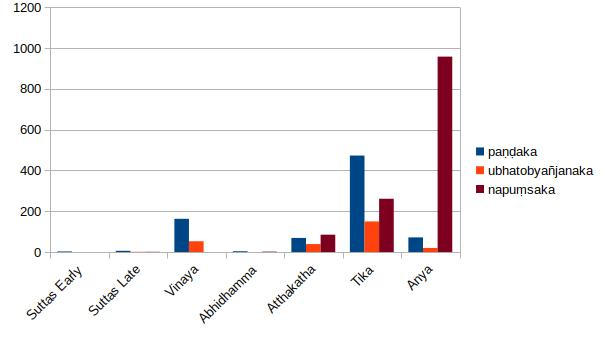
\includegraphics[width=\linewidth]{pali.jpg}
\captionof{figure}{Frequency of words in the pali canon and commentaries}
\label{pali1}

\subsection{Sanskrit Buddhist and Vedic canon}

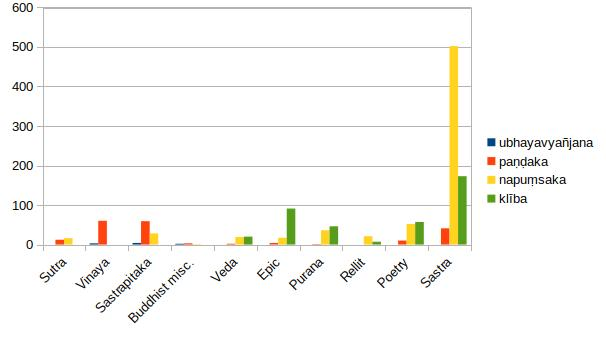
\includegraphics[width=\linewidth]{sanskrit.jpg}
\captionof{figure}{Frequency of words in the Sanskrit Buddhist and Vedic canon}
\label{sanskrit1}

\medskip
It is important to note that unlike the texts in the Pali canon, the search over the Sanskrit text only use the GRETIL database and do not comprise of the entire Buddhist canon. The Vedic canon is also included in this chart.


\subsection{Tibetan canon and commentaries}

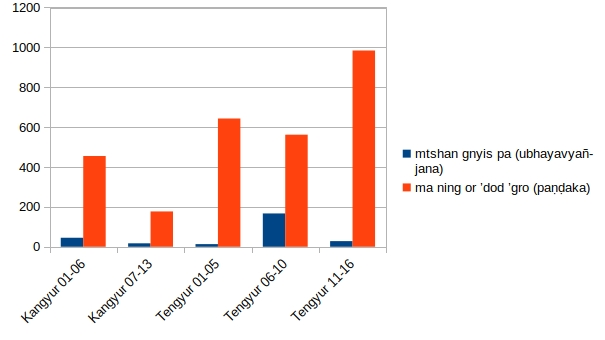
\includegraphics[width=\linewidth]{tibetan.jpg}
\captionof{figure}{Frequency of words in the tibetan canon and commentaries}
\label{tibetan1}



\newpage
\section{Analysis of the terms in the context of ordination}

The rule against ordination of both the {\em paṇḍaka } and the {\em ubhatob­yañ­janaka } are laid down in Khandaka 1 and are clearly against the full ordination of these two types of individuals, the {\em upasampadā}. Yet it is interesting that in both cases the person to whom the rule applies is said to have been given the {\em pabbajjā}. This really only makes sense if we understand {\em pabbajjā} here to be equivalent to {\em upasampadā}. In fact this equivalence between {\em pabbajjā} and {\em upasampadā} is what we find throughout the earliest Vinaya, and indeed the suttas \footnote{The {\em sāmaṇeras/īs} are barely mentioned in the suttas. Instead we find the figure of the {\em samaṇuddesa}, "one designated as a {\em samaṇa}", who seems to have had a looser affiliation with the Sangha, that is, no proper ordination. The commentaries glosses them as {\em sāmaṇeras}, but this might be an oversimplification. More likely they were a kind of precursor to the more formal status of novice. It seems likely that such people merely put on robes, and then lived in with loose connection to a particular community of ascetics, in which case their sex would have been a non-issue. I would argue it is natural to see novices proper in the same way. But the {\em samaṇuddesa} remains obscure.}. In any case, the rules itself are clearly limited to {\em upasampadā}.

\subsection{Paṇḍaka}

\begin{quote}
{\em Tena kho pana samayena aññataro paṇḍako bhikkhūsu \textbf{pabbajito} hoti. So dahare dahare bhikkhū upasaṅkamitvā evaṃ vadeti—“etha, maṃ āyasmanto dūsethā”ti. Bhikkhū apasādenti—“nassa, paṇḍaka, vinassa, paṇḍaka, ko tayā attho”ti. So bhikkhūhi apasādito mahante mahante moḷigalle sāmaṇere upasaṅkamitvā evaṃ vadeti—“etha, maṃ āvuso dūsethā”ti. Sāmaṇerā apasādenti—“nassa, paṇḍaka, vinassa, paṇḍaka, ko tayā attho”ti. So sāmaṇerehi apasādito hatthibhaṇḍe assabhaṇḍe upasaṅkamitvā evaṃ vadeti—“etha, maṃ āvuso dūsethā”ti. Hatthibhaṇḍā assabhaṇḍā dūsesuṃ. Te ujjhāyanti khiyyanti vipācenti—“paṇḍakā ime samaṇā sakyaputtiyā. Yepi imesaṃ na paṇḍakā, tepi ime paṇḍake dūsenti. Evaṃ ime sabbeva abrahmacārino”ti. Assosuṃ kho bhikkhū tesaṃ hatthibhaṇḍānaṃ assabhaṇḍānaṃ ujjhāyantānaṃ khiyyantānaṃ vipācentānaṃ. Atha kho te bhikkhū bhagavato etamatthaṃ ārocesuṃ. “Paṇḍako, bhikkhave, anupasampanno na \textbf{upasampādetabbo}, upasampanno nāsetabbo”ti. (Mahakkhandhaka, PTS 1.86)}
\end{quote}

\medskip

\begin{quote}
At one time a certain {\em paṇḍaka} had gone forth as a monk. He approached the young monks and said, “Venerables, come and have sex with me.”
The monks dismissed him, “Go away, {\em paṇḍaka}. Who needs you?”
\end{quote}
\begin{quote}
He went to the big and fat novices, said the same thing, and got the same response.
He then went to the elephant keepers and horse keepers, and once again he said the same thing. And they had sex with him. They complained and criticized them, “These Sakyan ascetics are {\em paṇḍaka}s. And those who are not have sex with them. None of them is celibate.”
\end{quote}
\begin{quote}
The monks heard their complaints. They told the Buddha and he said, “A {\em paṇḍaka} should not be given the full ordination. If it has been given, he should be expelled.”
\end{quote}



\subsection{Ubhatob­yañ­janaka}

\begin{quote}
{\em Tena kho pana samayena aññataro ubhatobyañjanako bhikkhūsu \textbf{pabbajito} hoti. So karotipi kārāpetipi. Bhagavato etamatthaṃ ārocesuṃ. Ubhatobyañjanako, bhikkhave, anupasampanno na upasampādetabbo, \textbf{upasampanno} nāsetabboti. (Mahakkhandhaka, PTS 1.89)}
\end{quote}

\medskip

\begin{quote}
At one time an {\em ubhatob­yañ­janaka} had gone forth as a monk. He had sex and made others have it.
\end{quote}
\begin{quote}
They told the Buddha and he said, “An {\em ubhatob­yañ­janaka} should not be given the full ordination. If it has been given, he should be expelled.”
\end{quote}

The commentary {\em (Samantapādādikā, vol. 3, para. 116)} mentions the following about {\em ubhatob­yañ­janaka}:

\begin{quote}
Ubhatobyañjanako ... so duvidho hoti – itthiubhatobyañjanako, purisaubhatobyañjanakoti. Tattha itthiubhatobyañjanakassa itthinimittaṃ pākaṭaṃ hoti, purisanimittaṃ paṭicchannaṃ. Purisaubhatobyañjanakassa purisanimittaṃ pākaṭaṃ, itthinimittaṃ paṭicchannaṃ. ... Imassa pana duvidhassāpi ubhatobyañjanakassa neva pabbajjā atthi, na upasampadāti
\end{quote}

\medskip

\begin{quote}
The {\em ubhatob­yañ­janaka} is of two sorts: the female {\em ubhatob­yañ­janaka} and the male {\em ubhatob­yañ­janaka}. For the female {\em ubhatob­yañ­janaka} the female characteristics are revealed, whereas the male characteristics are concealed. For the male {\em ubhatob­yañ­janaka} the male characteristics are revealed, whereas the female characteristics are concealed. ... 
\end{quote}
\begin{quote}
For either of these there is neither a going forth ({\em pabbajjā}) nor a full ordination ({\em upasampadā}).
\end{quote}

The commentary makes a distinction between male and female {\em ubhatob­yañ­janaka} whereby characteristics of the other sex are hidden. This is a much broader definition and a much broader subset of the term "intersex" as we know it today. The fact that they are predominantly male or female would be a fairly objective basis for deciding on ordination with the Bhikkhus or Bhikkhunis. This distinction is not mentioned in the Vinaya. But the commentary also makes a distinction between {\em pabbajjā} and {\em upasampadā} and does not allow either for ordination.





-------------------------------------------
One thing that struck me in Khandaka 1 is that both passages for paṇḍaka and ubhatobyañjanako deal with monks (already ordained!) having sex and therefore breaking Parajika 1. But instead of being rightfully expelled on those grounds for their bad behavior, they are expelled for who they ARE, together will a whole lot of other monks (at that time and in the future), who might be examplarery practitioners. The only other example of that in KD1 is animals but the origin story of that also seems rather more mythological than anything that actually happened. All the other examples of people not to be ordained are those who have such heavy defilements that they cannot either practise properly or would be a burden to the community because they might fall into the same bad habits again. So those people are not accepted because of what they have DONE. Having a certain body can hardly be regarded as a defilement, unless you look at it in the light of the idea of "past bad kamma". However, the Buddha never punished anybody for the way they were born.
This difference only makes sense if you read the translations according to a later interpretation of the words paṇḍaka and ubhatobyañjanako, namely people who have extremely strong sexual desire as I pointed out in my earlier article on pandakas. In fact, a eunuch has far less sexual desire as he no longer produces testosterone and there is no indication that an intersex person would have more sexual desire than other people. 



  "atk-vin02a20:323": "Ubhatobyañjanakavatthukathā",
  "atk-vin02a20:324": "116.Ubhatobyañjanako bhikkhaveti itthinimittuppādanakammato ca purisanimittuppādanakammato ca ubhato byañjanamassa atthīti ubhatobyañjanako. Karotīti purisanimittena itthīsu methunavītikkamaṁ karoti. Kārāpetīti paraṁ samādapetvā attano itthinimitte kārāpeti, so duvidho hoti – itthiubhatobyañjanako, purisaubhatobyañjanakoti.",
  "atk-vin02a20:325": "Tattha itthiubhatobyañjanakassa itthinimittaṁ pākaṭaṁ hoti, purisanimittaṁ paṭicchannaṁ. Purisaubhatobyañjanakassa purisanimittaṁ pākaṭaṁ, itthinimittaṁ paṭicchannaṁ. Itthiubhatobyañjanakassa itthīsu purisattaṁ karontassa itthinimittaṁ paṭicchannaṁ hoti, purisanimittaṁ pākaṭaṁ hoti. Purisaubhatobyañjanakassa purisānaṁ itthibhāvaṁ upagacchantassa purisanimittaṁ paṭicchannaṁ hoti, itthinimittaṁ pākaṭaṁ hoti. Itthiubhatobyañjanako sayañca gabbhaṁ gaṇhāti, parañca gaṇhāpeti. Purisaubhatobyañjanako pana sayaṁ na gaṇhāti, paraṁ gaṇhāpetīti, idametesaṁ nānākaraṇaṁ. Kurundiyaṁ pana vuttaṁ – ‘‘yadi paṭisandhiyaṁ purisaliṅgaṁ pavatte itthiliṅgaṁ nibbattati, yadi paṭisandhiyaṁ itthiliṅgaṁ pavatte purisaliṅgaṁ nibbattatī’’ti . Tattha vicāraṇakkamo vitthārato aṭṭhasāliniyā dhammasaṅgahaṭṭhakathāya veditabbo. Imassa pana duvidhassāpi ubhatobyañjanakassa neva pabbajjā atthi, na upasampadāti idamidha veditabbaṁ.",
  "atk-vin02a20:326": "Ubhatobyajjanakavatthukathā niṭṭhitā.",

Samantapasadika
Ubhatobyañjanako bhikkhaveti itthinimittuppādanakammato ca purisanimittuppādanakammato ca ubhato byañjanamassa atthīti ubhatobyañjanako.Karotīti purisanimittena itthīsu methunavītikkamaṃ karoti. Kārāpetīti paraṃ samādapetvā attano itthinimitte kārāpeti, so duvidho hoti – itthiubhatobyañjanako, purisaubhatobyañjanakoti.Tattha itthiubhatobyañjanakassa itthinimittaṃ pākaṭaṃ hoti, purisanimittaṃ paṭicchannaṃ. Purisaubhatobyañjanakassa purisanimittaṃ pākaṭaṃ, itthinimittaṃ paṭicchannaṃ. Itthiubhatobyañjanakassa itthīsu purisattaṃ karontassa itthinimittaṃ paṭicchannaṃ hoti, purisanimittaṃ pākaṭaṃ hoti. Purisaubhatobyañjanakassa purisānaṃ itthibhāvaṃ upagacchantassa purisanimittaṃ paṭicchannaṃ hoti, itthinimittaṃ pākaṭaṃ hoti. Itthiubhatobyañjanako sayañca gabbhaṃ gaṇhāti, parañca gaṇhāpeti. Purisaubhatobyañjanako pana sayaṃ na gaṇhāti, paraṃ gaṇhāpetīti, idametesaṃ nānākaraṇaṃ. 

Because of kamma giving rise to female characteristics and kamma giving rise to male characteristics, there is for them the characteristics of both. With the male characteristic they act to transgress through sexual intercourse with women. Having encouraged another, they cause action in their own female characteristic. 

[My comment: This seems to refer to a true hermaphrodite, assuming that such people even exist. The positive thing about this interpretation is that I am guessing very few people would be barred from ordaining.] 

They are twofold: the female ubhatobyañjanaka and the male ubhatobyañjanaka. In regard to this, the female characteristic of the female ubhatobyañjanaka is apparent, but the male characteristic is hidden. The male characteristic of the male ubhatobyañjanaka is apparent, but the female characteristic is hidden. 

While the female ubhatobyañjanaka is acting with manliness among women, the female characteristic is hidden, whereas the male characteristic is apparent. 
When the male ubhatobyañjanaka enters the state of a woman for the sake of men, the male characteristic is hidden, whereas the female characteristic is apparent. 
The female ubhatobyañjanaka becomes pregnant and causes others to become pregnant. The male ubhatobyañjanaka does not become pregnant, but causes others to become pregnant. This is the difference between them."



  "atk-vin02a20:277": "Paṇḍakavatthukathā",
  "atk-vin02a20:278": "109.Dahare dahareti taruṇe taruṇe. Moḷigalleti thūlasarīre. Hatthibhaṇḍe assabhaṇḍeti hatthigopake ca assagopake ca.",
  "atk-vin02a20:279": "Paṇḍakobhikkhaveti ettha āsittapaṇḍako usūyapaṇḍako opakkamikapaṇḍako pakkhapaṇḍako napuṁsakapaṇḍakoti pañca paṇḍakā. Tattha yassa paresaṁ aṅgajātaṁ mukhena gahetvā asucinā āsittassa pariḷāho vūpasammati, ayaṁ āsittapaṇḍako. Yassa paresaṁ ajjhācāraṁ passato usūyāya uppannāya pariḷāho vūpasammati, ayaṁ usūyapaṇḍako. Yassa upakkamena bījāni apanītāni, ayaṁ opakkamikapaṇḍako. Ekacco pana akusalavipākānubhāvena kāḷapakkhe paṇḍako hoti, juṇhapakkhe panassa pariḷāho vūpasammati, ayaṁ pakkhapaṇḍako. Yo pana paṭisandhiyaṁyeva abhāvako uppanno, ayaṁ napuṁsakapaṇḍakoti. Tesu āsittapaṇḍakassa ca usūyapaṇḍakassa ca pabbajjā na vāritā, itaresaṁ tiṇṇaṁ vāritā. Tesupi pakkhapaṇḍakassa yasmiṁ pakkhe paṇḍako hoti, tasmiṁyevassa pakkhe pabbajjā vāritāti kurundiyaṁ vuttaṁ. Yassa cettha pabbajjā vāritā, taṁ sandhāya idaṁ vuttaṁ – ‘‘anupasampanno na upasampādetabbo upasampanno nāsetabbo’’ti. Sopi liṅganāsaneneva nāsetabbo. Ito paraṁ ‘‘nāsetabbo’’ti vuttesupi eseva nayo.",
  "atk-vin02a20:280": "Paṇḍavatthukathā niṭṭhitā.",

  https://web.archive.org/web/20170404051712/http://www.australianhumanitiesreview.org/archive/issue1-feb-mar-96/jackson/references.html translates and explain these pandaka terms
\newpage
\bibliographystyle{plainnat}
\bibliography{bib}


\end{document}

